%%
%% This is file `chapmin.tex',
%% generated with the docstrip utility.
%%
%% The original source files were:
%%
%% ths.dtx  (with options: `chapmin')
%% 
%% IMPORTANT NOTICE:
%% 
%% For the copyright see the source file.
%% 
%% Any modified versions of this file must be renamed
%% with new filenames distinct from chapmin.tex.
%% 
%% For distribution of the original source see the terms
%% for copying and modification in the file ths.dtx.
%% 
%% This generated file may be distributed as long as the
%% original source files, as listed above, are part of the
%% same distribution. (The sources need not necessarily be
%% in the same archive or directory.)


\section{Mathmatic Development}

Where does this text go?

\subsection{The Boltzmann Equation}

The time dependent gamma transport equation can be written as

\begin{equation} \label{eq:boltz_t_dep}
\begin{split}
	&\left[ \frac{1}{v(E)} \frac{\partial}{\partial t} + \hat{\Omega} \cdot \nabla + \Sigma_t(\boldsymbol{r}, E, t) \right]
	\psi(\boldsymbol{r}, E, \hat{\Omega}, t) = \\
	&\int_{4 \pi} \int_0^\infty \Sigma_s(\boldsymbol{r}, E' \rightarrow E, \hat{\Omega}' \rightarrow \hat{\Omega}, t) \psi(\boldsymbol{r}, E', \hat{\Omega}', t) dE' d\hat{\Omega}' + S(\boldsymbol{r}, E, \hat{\Omega}, t)
\end{split}
\end{equation}

However, we are typically not concerned with the transient case in medical diagnostic imaging. We are more interested in the steady state case. The time independent form of Eq. \ref{eq:boltz_t_dep} is written as

\begin{equation} \label{eq:boltz}
\begin{split}
	&\left[ \hat{\Omega} \cdot \nabla + \Sigma_t(\boldsymbol{r}, E) \right]
	\psi(\boldsymbol{r}, E, \hat{\Omega}) = \\
	&\int_{4 \pi} \int_0^\infty \Sigma_s(\boldsymbol{r}, E' \rightarrow E, \hat{\Omega}' \rightarrow \hat{\Omega}) \psi(\boldsymbol{r}, E', \hat{\Omega}') dE' d\hat{\Omega}' + S(\boldsymbol{r}, E, \hat{\Omega})
\end{split}
\end{equation}

The following sections show how Eq.~\ref{eq:boltz} is discretized.

\subsection{Angular Discretization}
The coordinate system used in DOCTORS is shown in Fig.~\ref{fig:coord_sys}. A discrete set of $N_a$ angles ($\Omega_{a} \quad a = 0 \ldots N_a-1$) is selected to represent continuous directional space. Particles are transported only along these discrete directions form one voxel to adjacent voxels.

The $S_N$ quadrature is implemented in DOCTORS. There are many different quadrature sets, the $S_N$ quadratures were selected because they are easy to implement, rotationally symmetric, and the most commonly used in production discrete ordinate solvers. This enables simple, direct comparison to other solvers. Arbitrary quadratures are permissible in a plain text file supplied by the user enabling other quadratures.

\begin{figure}[tb]
  \begin{center}
   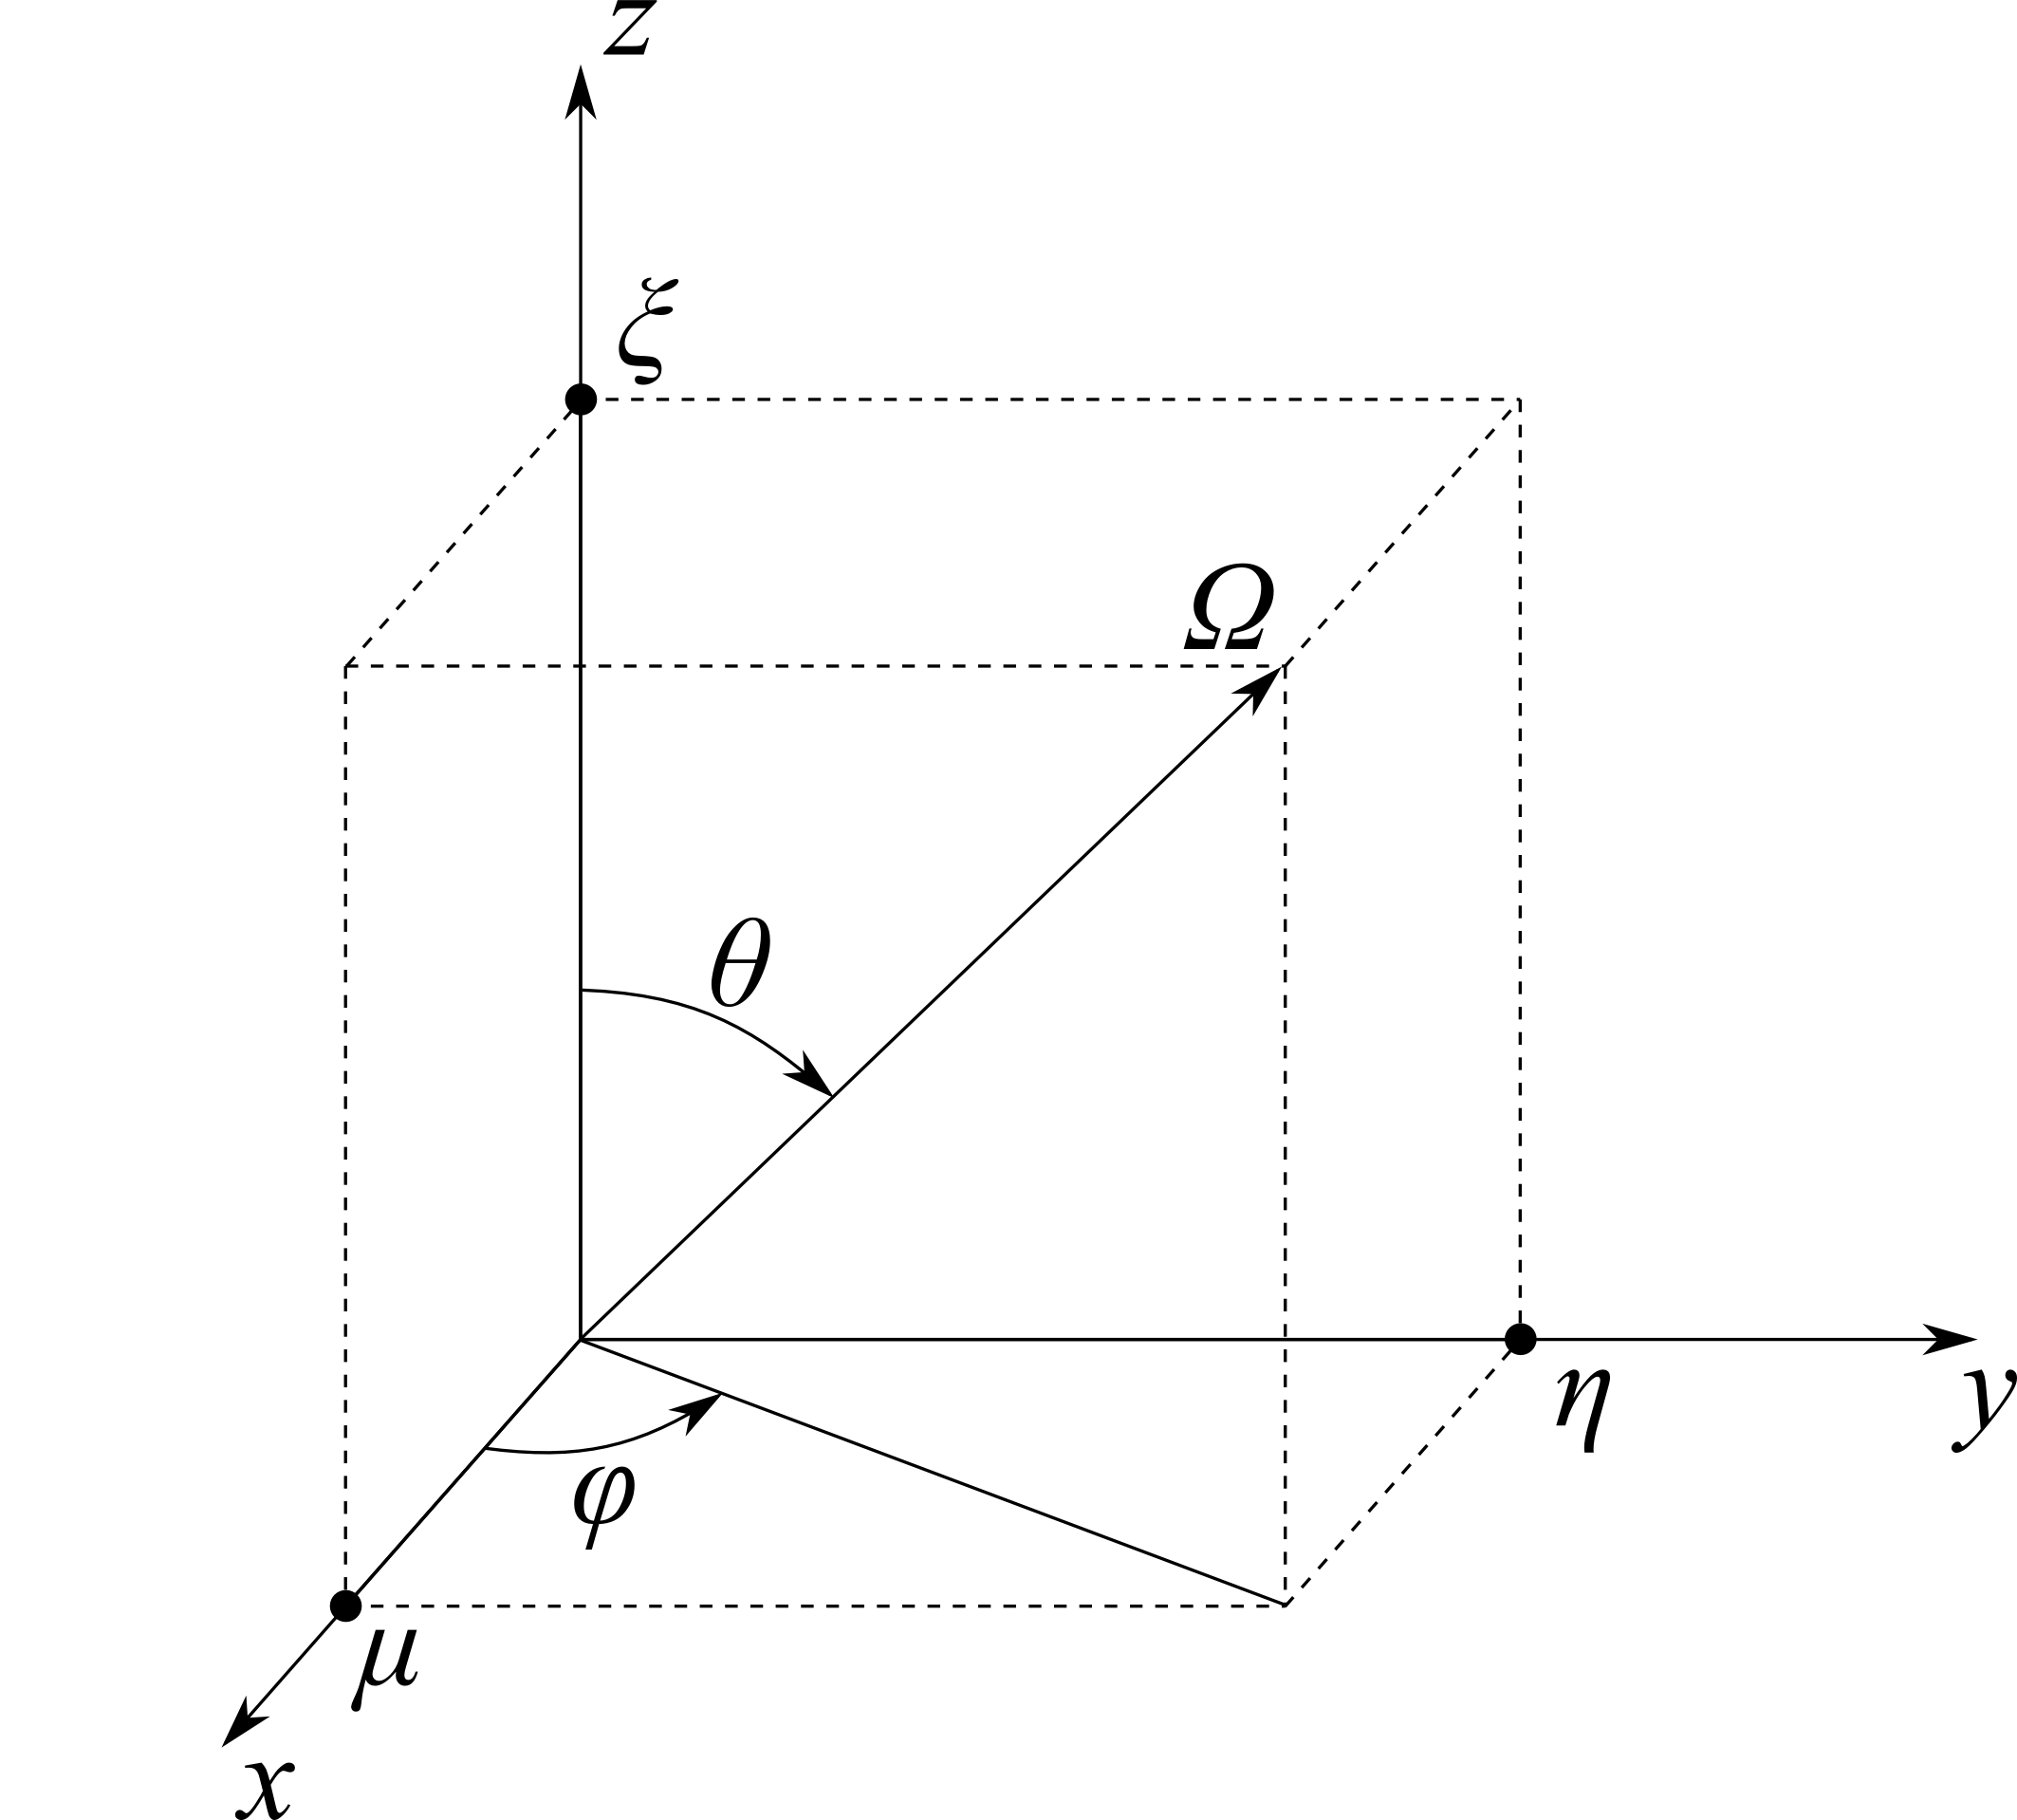
\includegraphics[width=3.75in]{figs/coord_sys}
  \end{center}
  \caption{The coordinate system used in DOCTORS. Given an arbitrary direction, $\Omega$, $\mu$, $\eta$, and $\xi$ are its direction cosines with respect to the $x$, $y$, and $z$ axes respectively. $\varphi$ is the azimuthal angle (with respect to $x$ and the d $\theta$ is the polar angle (with respect to $z$).}
\label{fig:coord_sys}
\end{figure}%

A given direction, $\hat{\Omega}$ is determined by its three cosine components. This relation is given in Eq.~\ref{eq:omega_cos} where $\hat{i}$, $\hat{j}$, and $\hat{k}$ are the unit directions in the $x$, $y$, and $z$ directions respectively.

\begin{equation} \label{eq:omega_cos}
	\hat{\Omega} = \mu \hat{i} + \eta \hat{j} + \xi \hat{k}
\end{equation}

Each discrete angle is associated a weight. The weights are designed with the angles such that once a discrete quadrature is selected, integration over continuous space becomes integration in discrete space approximated by Eq.~\ref{eq:disc_int}.

\begin{equation} \label{eq:disc_int}
\int_{4 \pi} f(\hat{\Omega}) d\Omega \approx \sum_{a=0}^{N_a-1} f(\hat{\Omega}_a) \omega_a
\end{equation}

Discretizing Eq.~\ref{eq:boltz} in angular space gives Eq.~\ref{eq:boltz_a} where the angle is denoted by subscript $a$.

\begin{equation} \label{eq:boltz_a}
\begin{split}
&\left[ \hat{\Omega}_a \cdot \nabla + \Sigma_t(\boldsymbol{r}, E) \right]
\psi_{a}(\boldsymbol{r}, E) = \\
&\sum_{a=0}^{N_a-1} \int_0^\infty \Sigma_{s, a, a'}(\boldsymbol{r}, E' \rightarrow E) \psi_{a'}(\boldsymbol{r}, E') dE' \omega_a + S_a(\boldsymbol{r}, E)
\end{split}
\end{equation}

\subsection{Energy Discretization}

Continuous energy is discretized into $G$ groups indexed from 0 to $G-1$. Upscatter is assumed to be negligible. Therefore, Eq.~\ref{eq:boltz_a} becomes the energy discretized Eq.~\ref{eq:boltz_e} where the group number is indexed by superscript $g$. The group structure is shown in Fig.~\ref{fig:energy_groups}.

\begin{equation} \label{eq:boltz_e}
\left[ \hat{\Omega}_a \cdot \nabla + \Sigma_t^g(\boldsymbol{r}) \right]
\psi_{a}^{g}(\boldsymbol{r}) = 
\sum_{a=0}^{N_a-1} \sum_{g'=g}^{G-1} \Sigma_{s, a, a'}^{g, g'}(\boldsymbol{r}) \psi_{a'}^{g'}(\boldsymbol{r}) \omega_a + S_a^g(\boldsymbol{r})
\end{equation}

\begin{figure}[tb]
  \begin{center}
   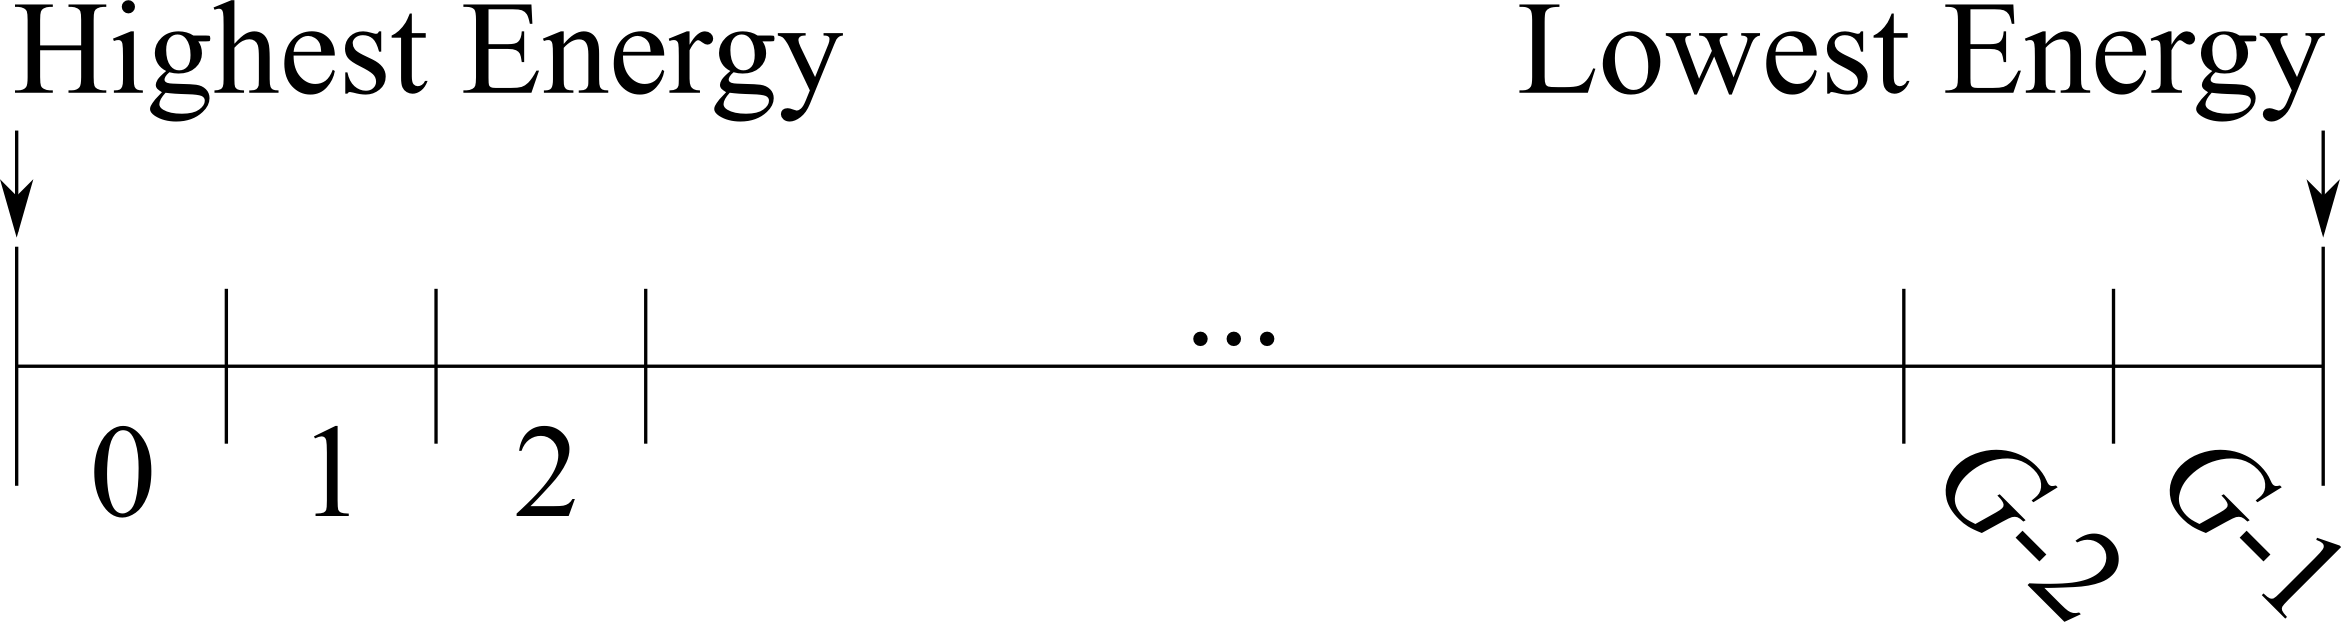
\includegraphics[width=3.75in]{figs/energy_groups}
  \end{center}
  \caption{The energy grid structure used in DOCTORS. The highest energy group is group 0 and the lowest energy is group $G-1$.}
\label{fig:energy_groups}
\end{figure}%

\subsection{Spatial Discretization}

Finally, Eq.~\ref{eq:boltz_e} is discretized in space to give Eq.~\ref{eq:boltz_r} which is fully discretized. The problem domain is split into an evenly spaced Cartesian grid. The grid spacing between each of the spatial dimensions does not necessarily need to be uniform, but it often is in the case of CT voxel phantoms.

The problem domain must be a regular rectangular parallelpiped of size $D_x$, $D_y$, and $D_z$ in the $x$, $y$, and $z$ directions respectively. The mesh is partitioned into $N_x$, $N_y$, and $N_z$ evenly spaced bins along each direction. The total number of voxels, $N_V$ is easily computed as the multiple of each of the component directions given in Eq.~\ref{eq:n_v}.

\begin{equation} \label{eq:n_v}
	N_V = N_x N_y N_z
\end{equation}

Voxel indices are flattened according to the rule given in Eq.~\ref{eq:indx_flat}. Note that all indeces always start at zero.

\begin{equation} \label{eq:indx_flat}
	i = i_x (N_z + N_y) + i_y N_z + i_z
\end{equation}

The spatial mesh is shown in Fig.~\ref{fig:spatial_disc}. The size of each voxel in each dimension is computed by dividing the size of the problem domain along in that dimension by the number of mesh elements along the same direction. Eq.~\ref{eq:mesh_x} shows this computation for the $x$ direction. Analagous equations apply in the $y$ and $z$ directions as well.

\begin{equation} \label{eq:mesh_x}
\Delta x = \frac{D_x}{N_x}
\end{equation}

\begin{figure}[tb]
  \begin{center}
   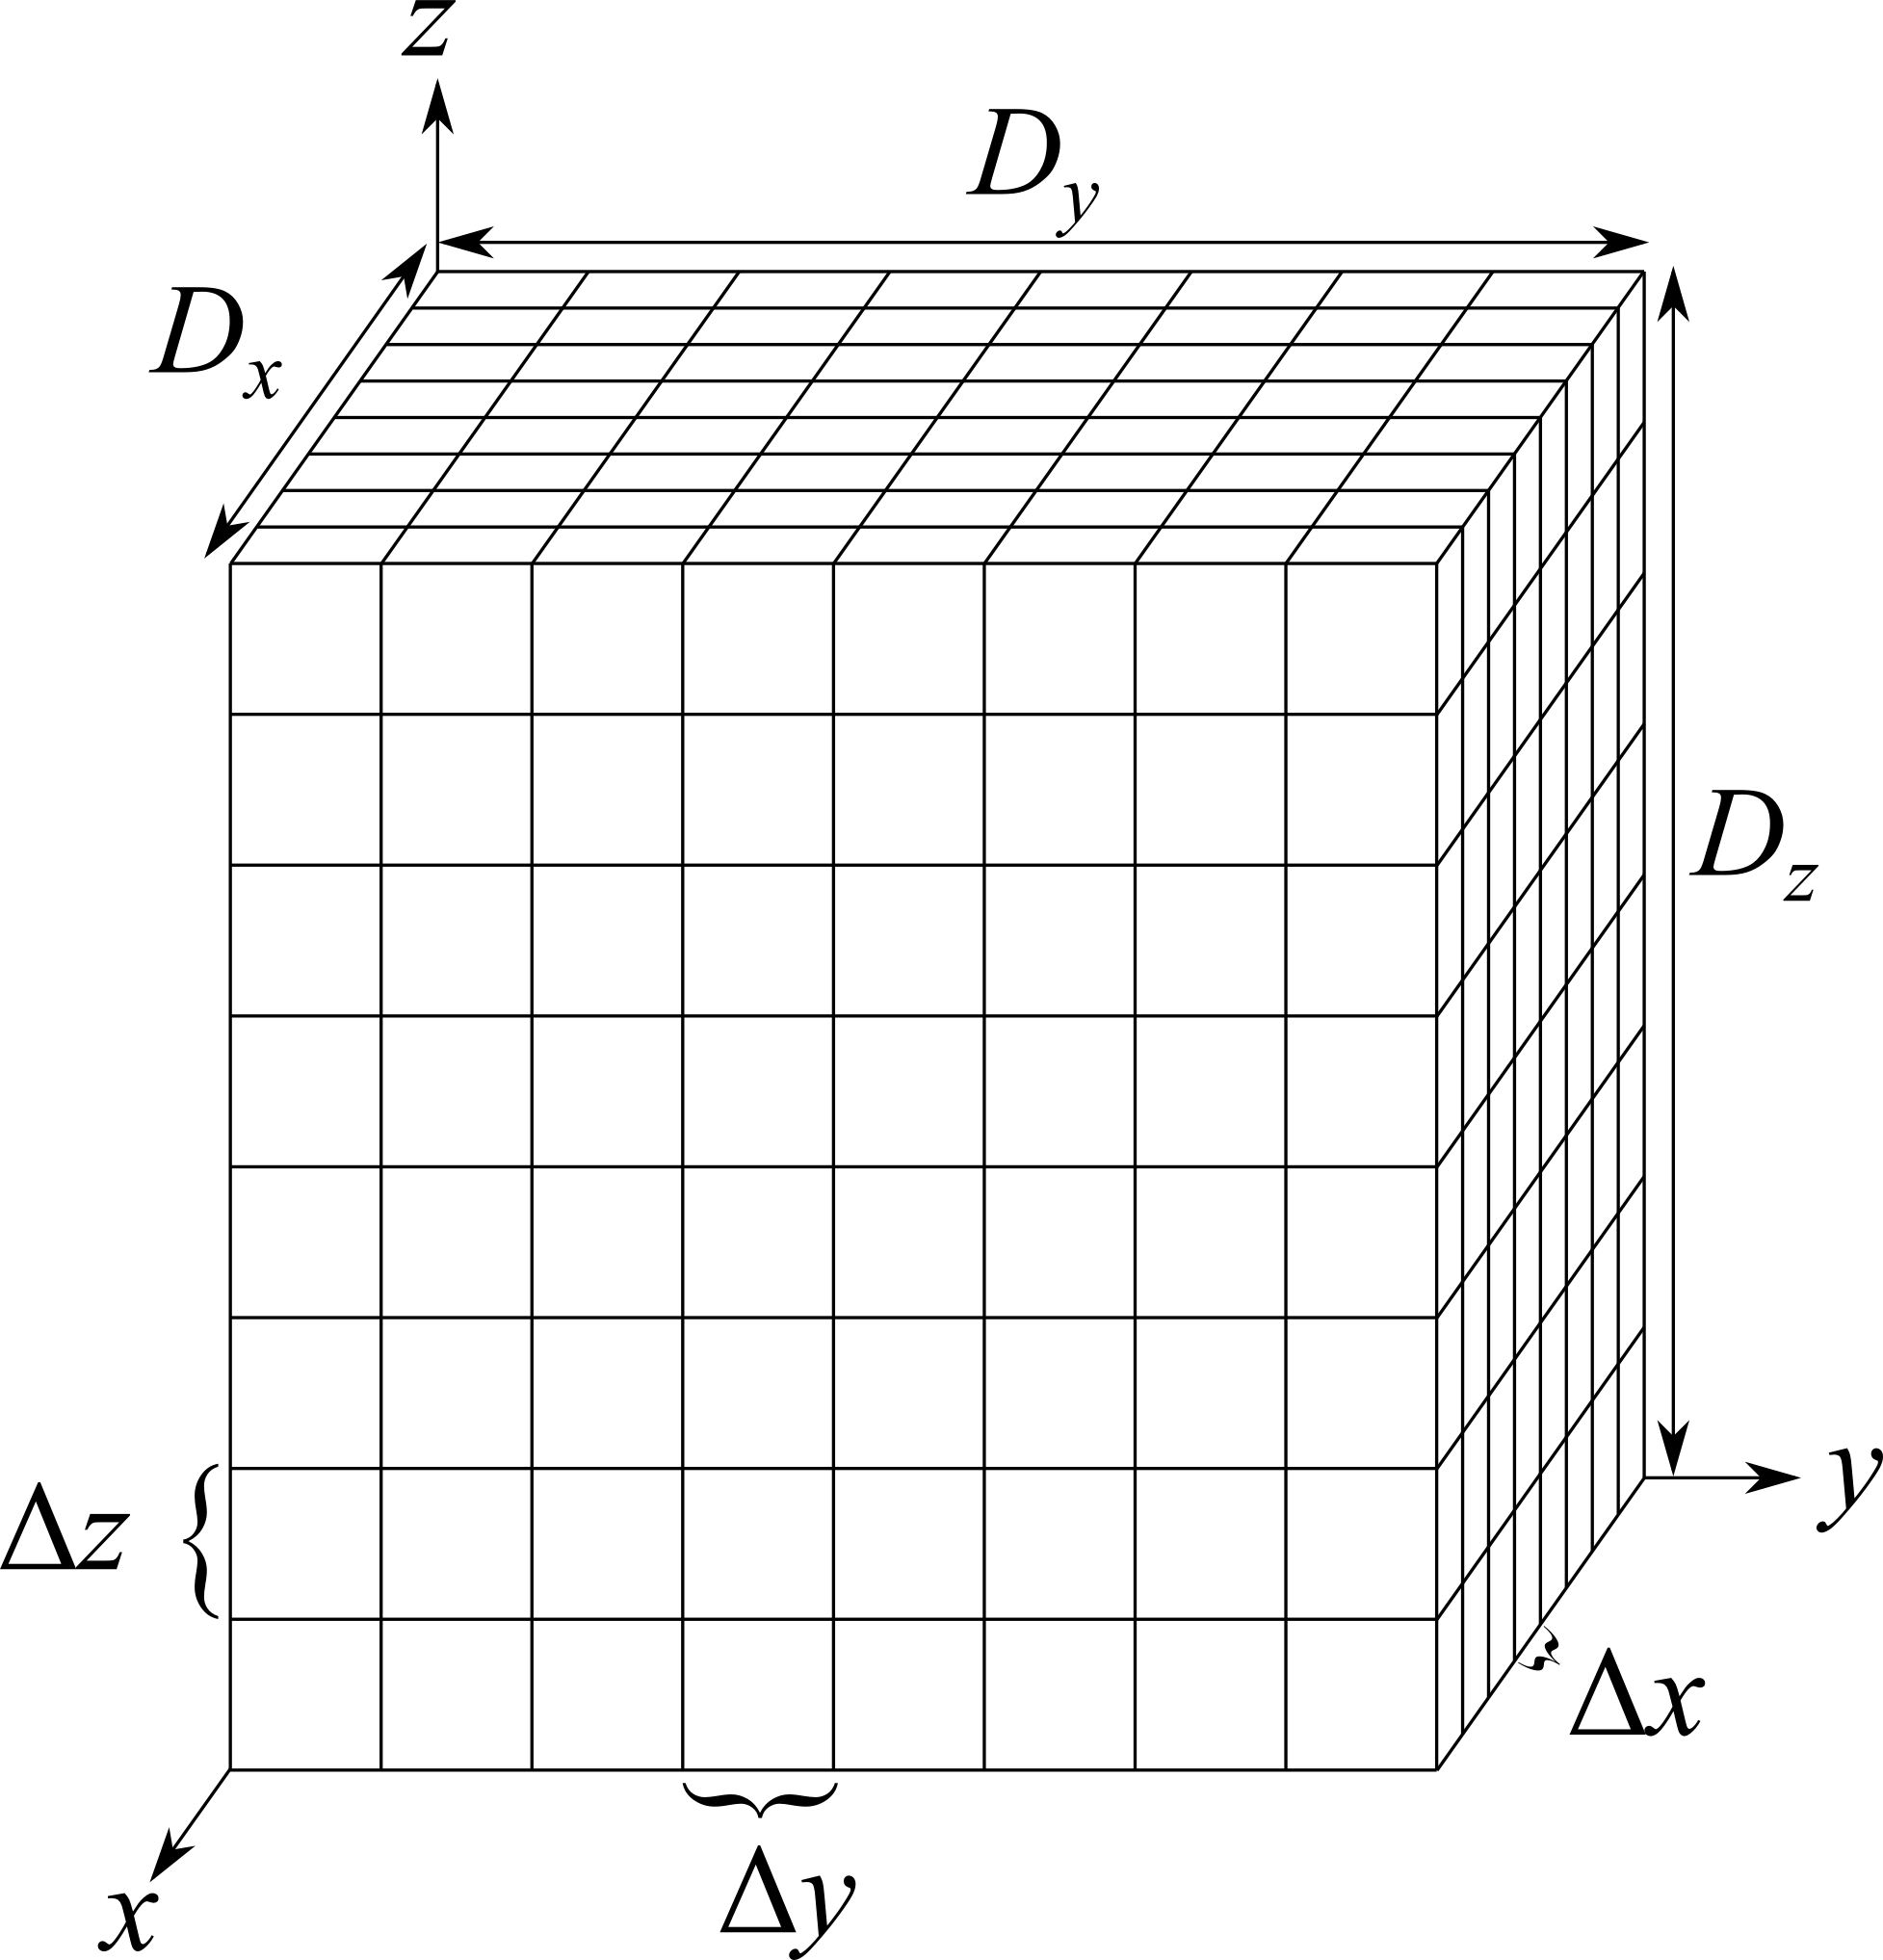
\includegraphics[width=3.75in]{figs/spatial_disc}
  \end{center}
  \caption{The spatial mesh imposed on the problem domain.}
\label{fig:spatial_disc}
\end{figure}%

The index of interest is denoted as a subscript $i$ which makes the fully discretized form of the steady state Linear Boltzmann Equation given in Eq.~\ref{eq:boltz} into the fully discretized form given in Eq.~\ref{eq:boltz_i}

\begin{equation} \label{eq:boltz_i}
\left[ \hat{\Omega}_a \cdot \nabla + \Sigma_{t,i}^g \right]
\psi_{i,a}^{g} = 
\sum_{a=0}^{N_a-1} \sum_{g'=g}^{G-1} \Sigma_{s, i, a, a'}^{g, g'} \psi_{i, a'}^{g'} \omega_a + S_{i,a}^g
\end{equation}

\subsection{Solution}

To solve the fully discretized form of the Linear Boltzmann Equation given in Eq.~\ref{eq:boltz_i}, the gradient operator must first be computed numerically. Recall that $\Omega_a$ can be written in vector notation using its cosine components as defined in Eq.~\ref{eq:omega_cos}. Also recall the definition of the gradient, given in Eq.~\ref{eq:grad}.

\begin{equation} \label{eq:grad}
\nabla f(x, y, z) = \frac{\partial f(x, y, z)}{\partial x} \hat{i} + \frac{\partial f(x, y, z)}{\partial y} \hat{j} + \frac{\partial f(x, y, z)}{\partial z} \hat{k}
\end{equation}

To the first order, a partial derivitive can be computed using Eq.~\ref{eq:deriv_1}.

\begin{equation} \label{eq:deriv_1}
\frac{\partial f(x)}{\partial x} \approx \frac{f(x) - f(x + \Delta x)}{\Delta x}
\end{equation}

Using the definition of $\Omega$ and Eq.~\ref{eq:grad} the $\hat{\Omega} \cdot \nabla \psi$ term can be rewritten using Eq.~\ref{eq:spatial_1}

\begin{equation} \label{eq:deriv_1}
\begin{split}
\Omega \cdot \nabla \psi & \approx 
\left\langle \mu, \eta, \xi \right\rangle \cdot
\left\langle \frac{\psi(x) - \psi(x + \Delta x)}{\Delta x},
\frac{\psi(y + \Delta y) - \psi(y)}{\Delta y},
\frac{\psi(z + \Delta z) - \psi(z)}{\Delta z} \right\rangle \\
& \approx 
\frac{\psi(x + \Delta x) - \psi(x)}{\Delta x} \mu + 
\frac{\psi(y + \Delta y) - \psi(y)}{\Delta y} \eta + 
\frac{\psi(z + \Delta z) - \psi(z)}{\Delta z} \xi
\end{split}
\end{equation}

Along some direction, $\Omega$, as it enters an arbitrary voxel, it must pass through either of the sides indicated in red and exit via the other as shown in Fig.~\ref{fig:gradient}. Fig.~\ref{fig:gradient} uses the $yz$ faces of the voxel for illustration. If $\eta$ is positive, $\Omega$ will enter through the $x_i$ surface and exit through the $x_{i+1}$ surface. If $\eta$ is negative, this order will be reversed. A limitation to this methodology is that $\mu$, $\eta$, and $\xi$ are assumed to be nonzero. This is ensured as long as none of the directions in the quadrature are parallel to a major axis.

\begin{figure}[tb]
  \begin{center}
   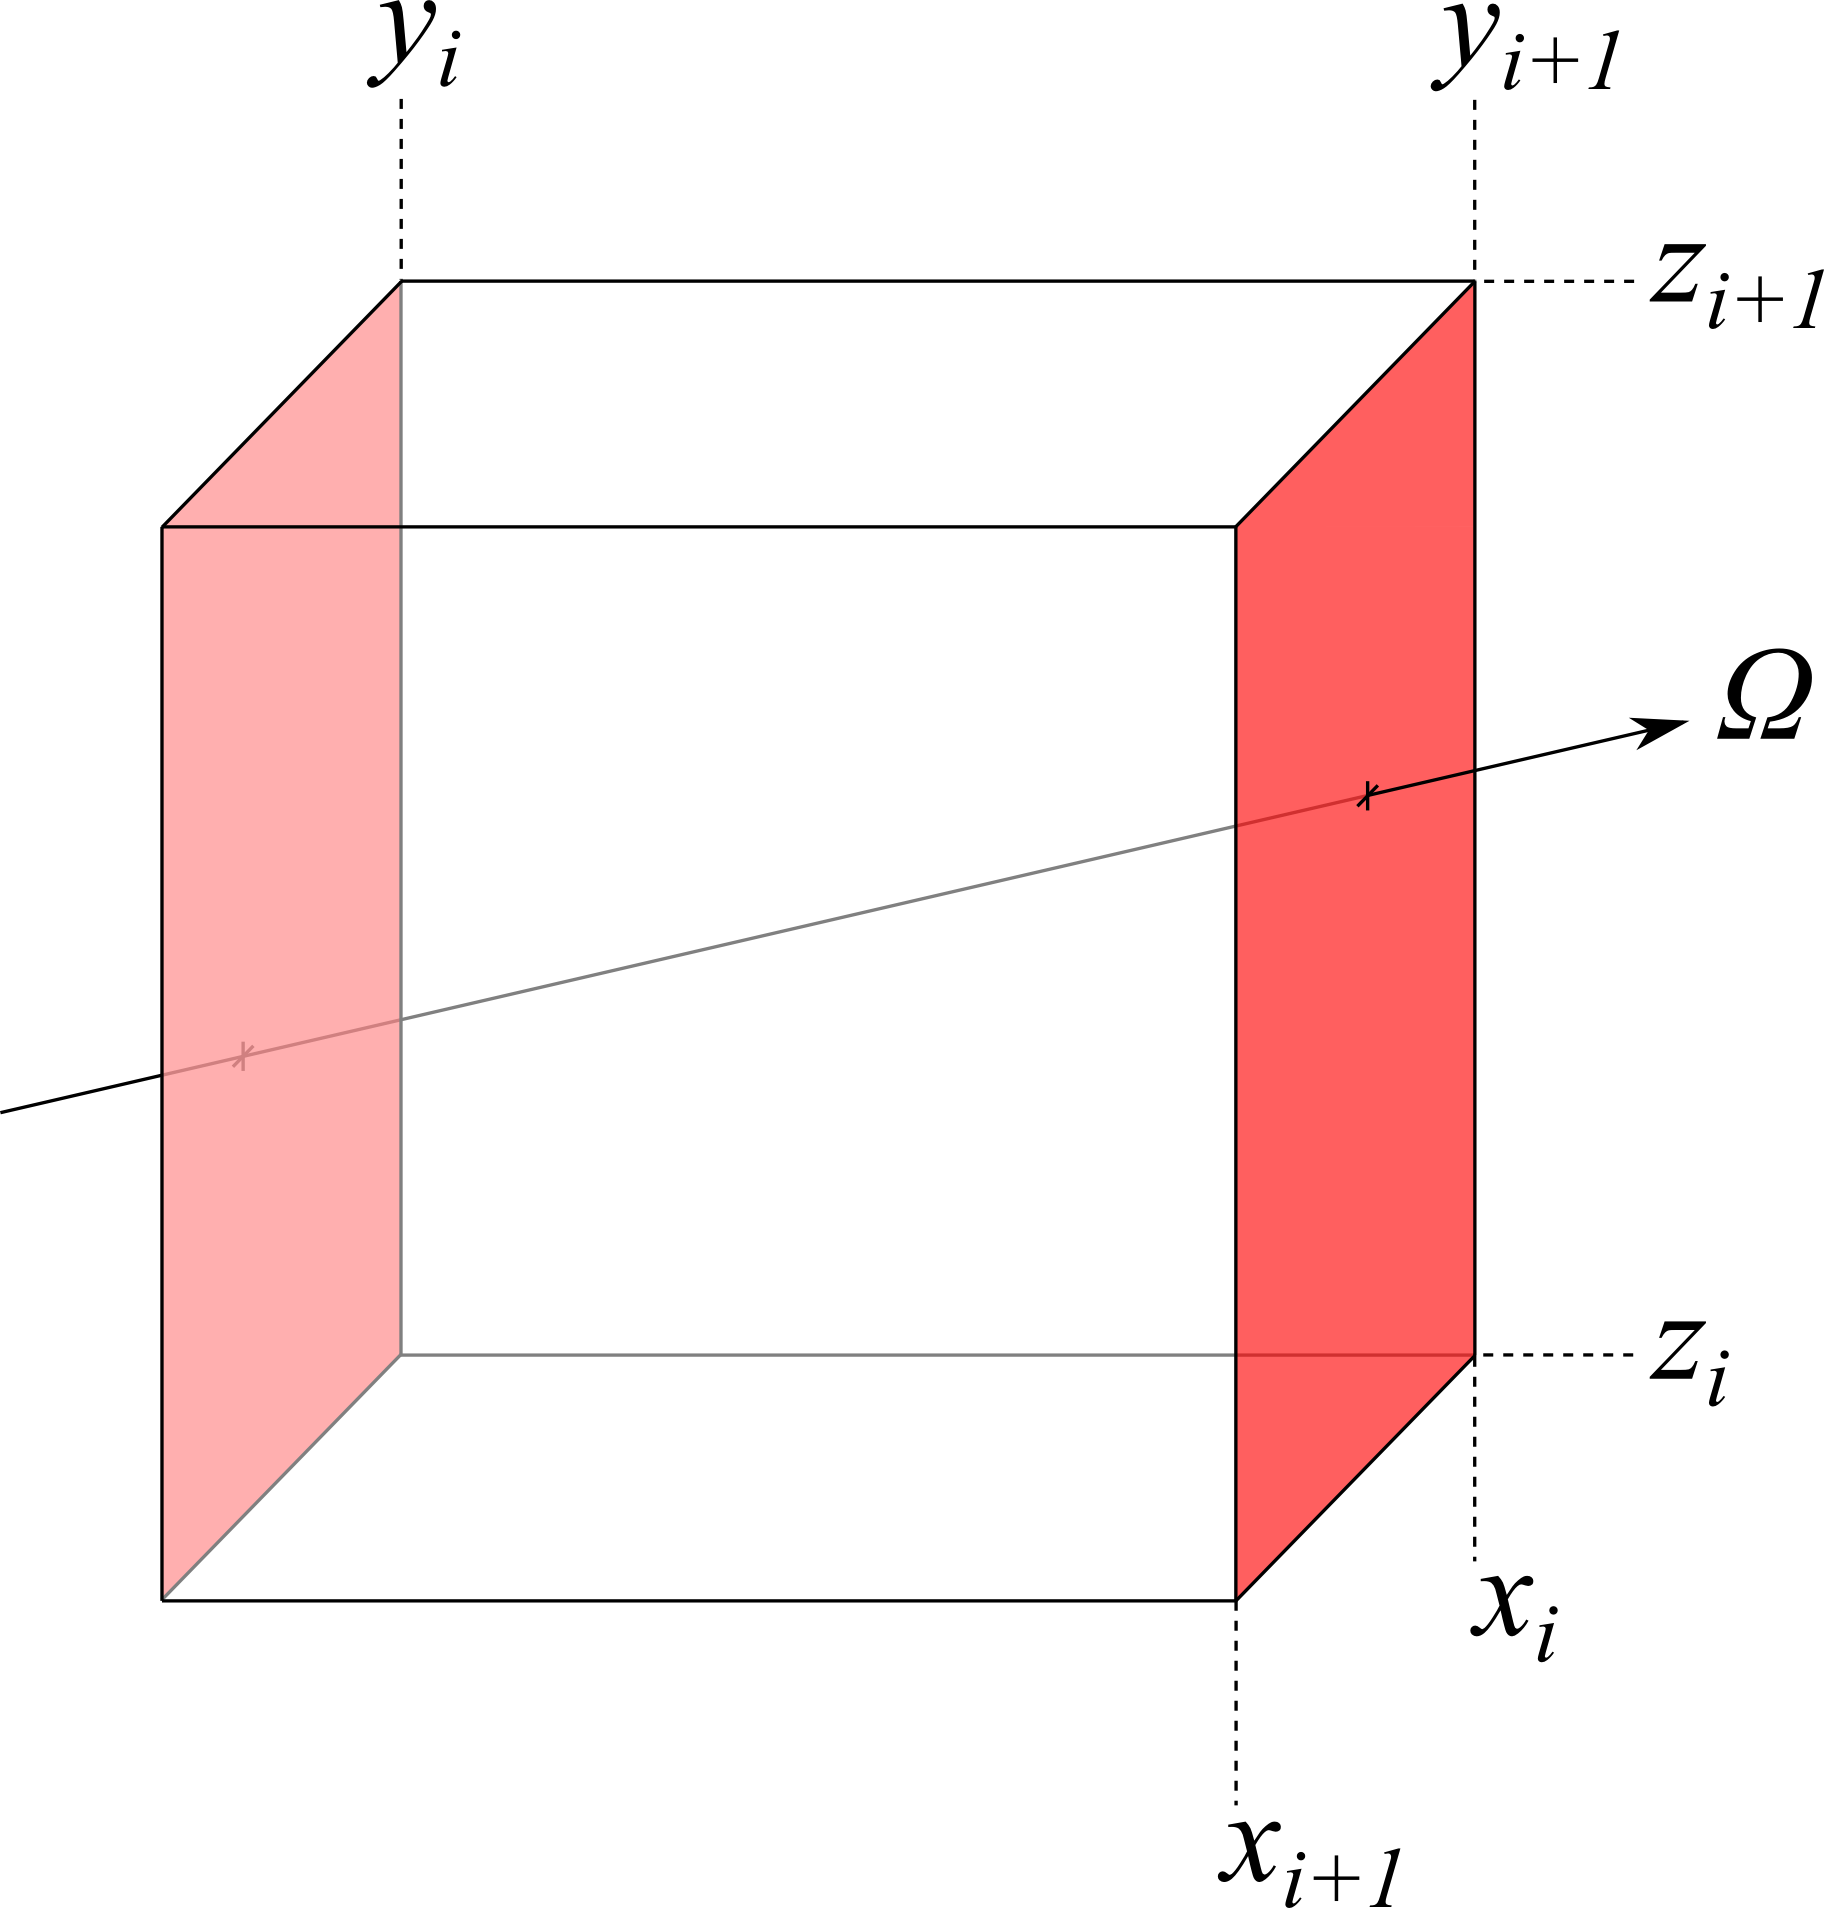
\includegraphics[width=3.75in]{figs/gradient}
  \end{center}
  \caption{The caption.}
\label{fig:gradient}
\end{figure}%

Depending on the sign of $\eta$, the first order approximation of the a derivitive along the $y$ direction is given by Eq.~\ref{eq:grad_y}.

\begin{equation} \label{eq:grad_y}
\begin{split}
\frac{\partial f}{\partial y} &= \frac{f(x_i) - f(x_{i+1})}{\Delta x}, \quad \eta>0 \\
\frac{\partial f}{\partial y} &= \frac{f(x_{i+1}) - f(x_{i})}{\Delta x}, \quad \eta <0 \\
\frac{\partial f}{\partial y} &= 0, \quad \eta=0
\end{split}
\end{equation}

Equation~\ref{eq:grad_y} can be generalized to use $f_{in}$ and $f_{out}$ instead of relying on the $x$-coordinate. This is given in Eq.~\ref{eq:grad_y2}

\begin{equation} \label{eq:grad_y2}
\begin{split}
\frac{\partial f}{\partial y} &= \frac{f_{in} - f_{out}}{\Delta x}, \quad \eta \neq 0 \\
\frac{\partial f}{\partial y} &= 0, \quad \eta=0
\end{split}
\end{equation}

The generalization of Eq.~\ref{eq:grad_y2} is applied to Eq.~\ref{eq:deriv_1} to yield Eq.~\ref{eq:deriv_2} which is generally valid for all octants.

\begin{equation} \label{eq:deriv_2}
\Omega \cdot \nabla \psi \approx 
\frac{\psi_{x,in} - \psi_{x,out}}{\Delta x} \mu + 
\frac{\psi_{y,in} - \psi_{y,out}}{\Delta y} \eta + 
\frac{\psi_{z,in} - \psi_{z,out}}{\Delta z} \xi
\end{equation}

Using the approximation given in Eq.~\ref{eq:deriv_2}, Eq.~\ref{eq:boltz_i} can be rewritten as Eq.~\ref{eq:boltz_i2}.

\begin{equation} \label{eq:boltz_i2}
\left[ 
\frac{\psi_{i,a,x,in}^g - \psi_{i,a,x,out}^g}{\Delta x} \mu + 
\frac{\psi_{i,a,y,in}^g - \psi_{i,a,y,out}^g}{\Delta y} \eta + 
\frac{\psi_{i,a,z,in}^g - \psi_{i,a,z,out}^g}{\Delta z} \xi
\right]
+ \Sigma_{t,i}^g \psi_{i,a}^{g} = 
\sum_{a=0}^{N_a-1} \sum_{g'=g}^{G-1} \Sigma_{s, i, a, a'}^{g, g'} \psi_{i, a'}^{g'} \omega_a + S_{i,a}^g
\end{equation}

It is useful to point out that each of $\psi_{i,a,x,in}^g$, $\psi_{i,a,x,out}^g$, $\psi_{i,a,y,in}^g$, $\psi_{i,a,y,out}^g$, $\psi_{i,a,z,in}^g$, and $\psi_{i,a,z,out}^g$ are \textit{surface} flux values while $\psi_{i,a}^{g}$ is a \textit{volume averaged} flux value.

In order for the discretized Linear Boltzmann Equation to be solved using Eq.~\ref{eq:boltz_i2}, the incoming flux must always be known. Either the boundary conditions or previously calculated values are used to determine each incoming flux. Therefore, in order to compute the average flux in a cell, some relationship between the average flux and the outgoing surface fluxes must be known. These values can be related by any one of many different mechanisms, the most common of which is the diamond difference approximation.

\subsection{Diamond Difference Approximation}

In the diamond difference approximation, it is assumed that the incoming and outgoing flux are both known. The average flux is assumed to be the average of the two surface fluxes. This is assumed to be the case in all three spatial dimensions. This leads to Eq.~\ref{eq:dd}.

\begin{equation} \label{eq:dd}
\begin{split}
\frac{\psi_{i,a,x,in}^g + \psi_{i,a,x,out}^g}{2} &= \psi_{i,a}^{g} \\
\frac{\psi_{i,a,y,in}^g + \psi_{i,a,y,out}^g}{2} &= \psi_{i,a}^{g} \\
\frac{\psi_{i,a,z,in}^g + \psi_{i,a,z,out}^g}{2} &= \psi_{i,a}^{g}
\end{split}
\end{equation}

Multiplying both sides of Eq.~\ref{eq:dd} and subtracting twice the outgoing surface flux from each yields Eq.~\ref{eq:dd2}.

\begin{equation} \label{eq:dd2}
\begin{split}
\psi_{i,a,x,in}^g - \psi_{i,a,x,out}^g &= 2\psi_{i,a}^{g} - \psi_{i,a,x,out}^g \\
\psi_{i,a,y,in}^g - \psi_{i,a,y,out}^g &= 2\psi_{i,a}^{g} - \psi_{i,a,y,out}^g \\
\psi_{i,a,z,in}^g - \psi_{i,a,z,out}^g &= 2\psi_{i,a}^{g} - \psi_{i,a,z,out}^g
\end{split}
\end{equation}

The form of the left hand side of Eq.~\ref{eq:dd2} is the same as in Eq.~\ref{eq:boltz_i2}. This allows Eq.~\ref{eq:dd2} to be used to make a substitution in Eq.~\ref{eq:boltz_i2} that removes the dependence on the outgoing flux from discretized equation. After the substitution, Eq.~\ref{eq:boltz_i3} will arise.

\begin{equation} \label{eq:boltz_i3}
\left[ 
\frac{2\psi_{i,a}^{g} - \psi_{i,a,x,out}^g}{\Delta x} \mu + 
\frac{2\psi_{i,a}^{g} - \psi_{i,a,y,out}^g}{\Delta y} \eta + 
\frac{2\psi_{i,a}^{g} - \psi_{i,a,z,out}^g}{\Delta z} \xi
\right]
+ \Sigma_{t,i}^g \psi_{i,a}^{g} = 
\sum_{a=0}^{N_a-1} \sum_{g'=g}^{G-1} \Sigma_{s, i, a, a'}^{g, g'} \psi_{i, a'}^{g'} \omega_a + S_{i,a}^g
\end{equation}

The diamond difference approximation defined in Eq.~\ref{eq:dd} can also be rearranged to solve for each outgoing flux once the volume averaged flux is computed. The outgoing flux is given by Eq.~\ref{eq:dd3}.

\begin{equation} \label{eq:dd3}
\begin{split}
\psi_{i,a,x,out}^g &= 2\psi_{i,a}^{g} - \psi_{i,a,x,in}^g \\
\psi_{i,a,y,out}^g &= 2\psi_{i,a}^{g} - \psi_{i,a,y,in}^g \\
\psi_{i,a,z,out}^g &= 2\psi_{i,a}^{g} - \psi_{i,a,z,in}^g
\end{split}
\end{equation}

Rearranging Eq.~\ref{eq:boltz_i3} to factor out the volume averaged flux term yields Eq.~\ref{eq:boltz_i4}.

\begin{equation} \label{eq:boltz_i4}
\left[ 
\frac{2\psi_{i,a}^{g}}{\Delta x} \mu + 
\frac{2\psi_{i,a}^{g}}{\Delta y} \eta + 
\frac{2\psi_{i,a}^{g}}{\Delta z} \xi
\right] - 
\left[ 
\frac{2\psi_{i,a,x,out}^g}{\Delta x} \mu + 
\frac{2\psi_{i,a,y,out}^g}{\Delta y} \eta + 
\frac{2\psi_{i,a,z,out}^g}{\Delta z} \xi
\right]
+ \Sigma_{t,i}^g \psi_{i,a}^{g} = 
\sum_{a=0}^{N_a-1} \sum_{g'=g}^{G-1} \Sigma_{s, i, a, a'}^{g, g'} \psi_{i, a'}^{g'} \omega_a + S_{i,a}^g
\end{equation}

Equation~\ref{eq:boltz_i4} can be directly solved for the volume averaged flux. The result is given in Eq.~\ref{eq:boltz_i5}.

\begin{equation} \label{eq:boltz_i5}
\psi_{i,a}^{g} = 
\frac{
  \sum_{a=0}^{N_a-1} \sum_{g'=g}^{G-1} \Sigma_{s, i, a, a'}^{g, g'} \psi_{i,     a'}^{g'} \omega_a + 
  \left[ 
    \frac{2\psi_{i,a,x,out}^g}{\Delta x} \mu + 
    \frac{2\psi_{i,a,y,out}^g}{\Delta y} \eta + 
    \frac{2\psi_{i,a,z,out}^g}{\Delta z} \xi
  \right] + S_{i,a}^g
}{
  \frac{2\mu}{\Delta x}  + 
  \frac{2\eta}{\Delta y} + 
  \frac{2\xi}{\Delta z} + 
  \Sigma_{t,i}^g
}
\end{equation}

\subsection{Anisotropy Treatment}

Scatter is assumed to be a function of only the scatter angle between the initial and scattered directions, $\theta_s$. Often, the cosine of the scatter angle, $\mu_s$ is used.

\begin{figure}[tb]
  \begin{center}
   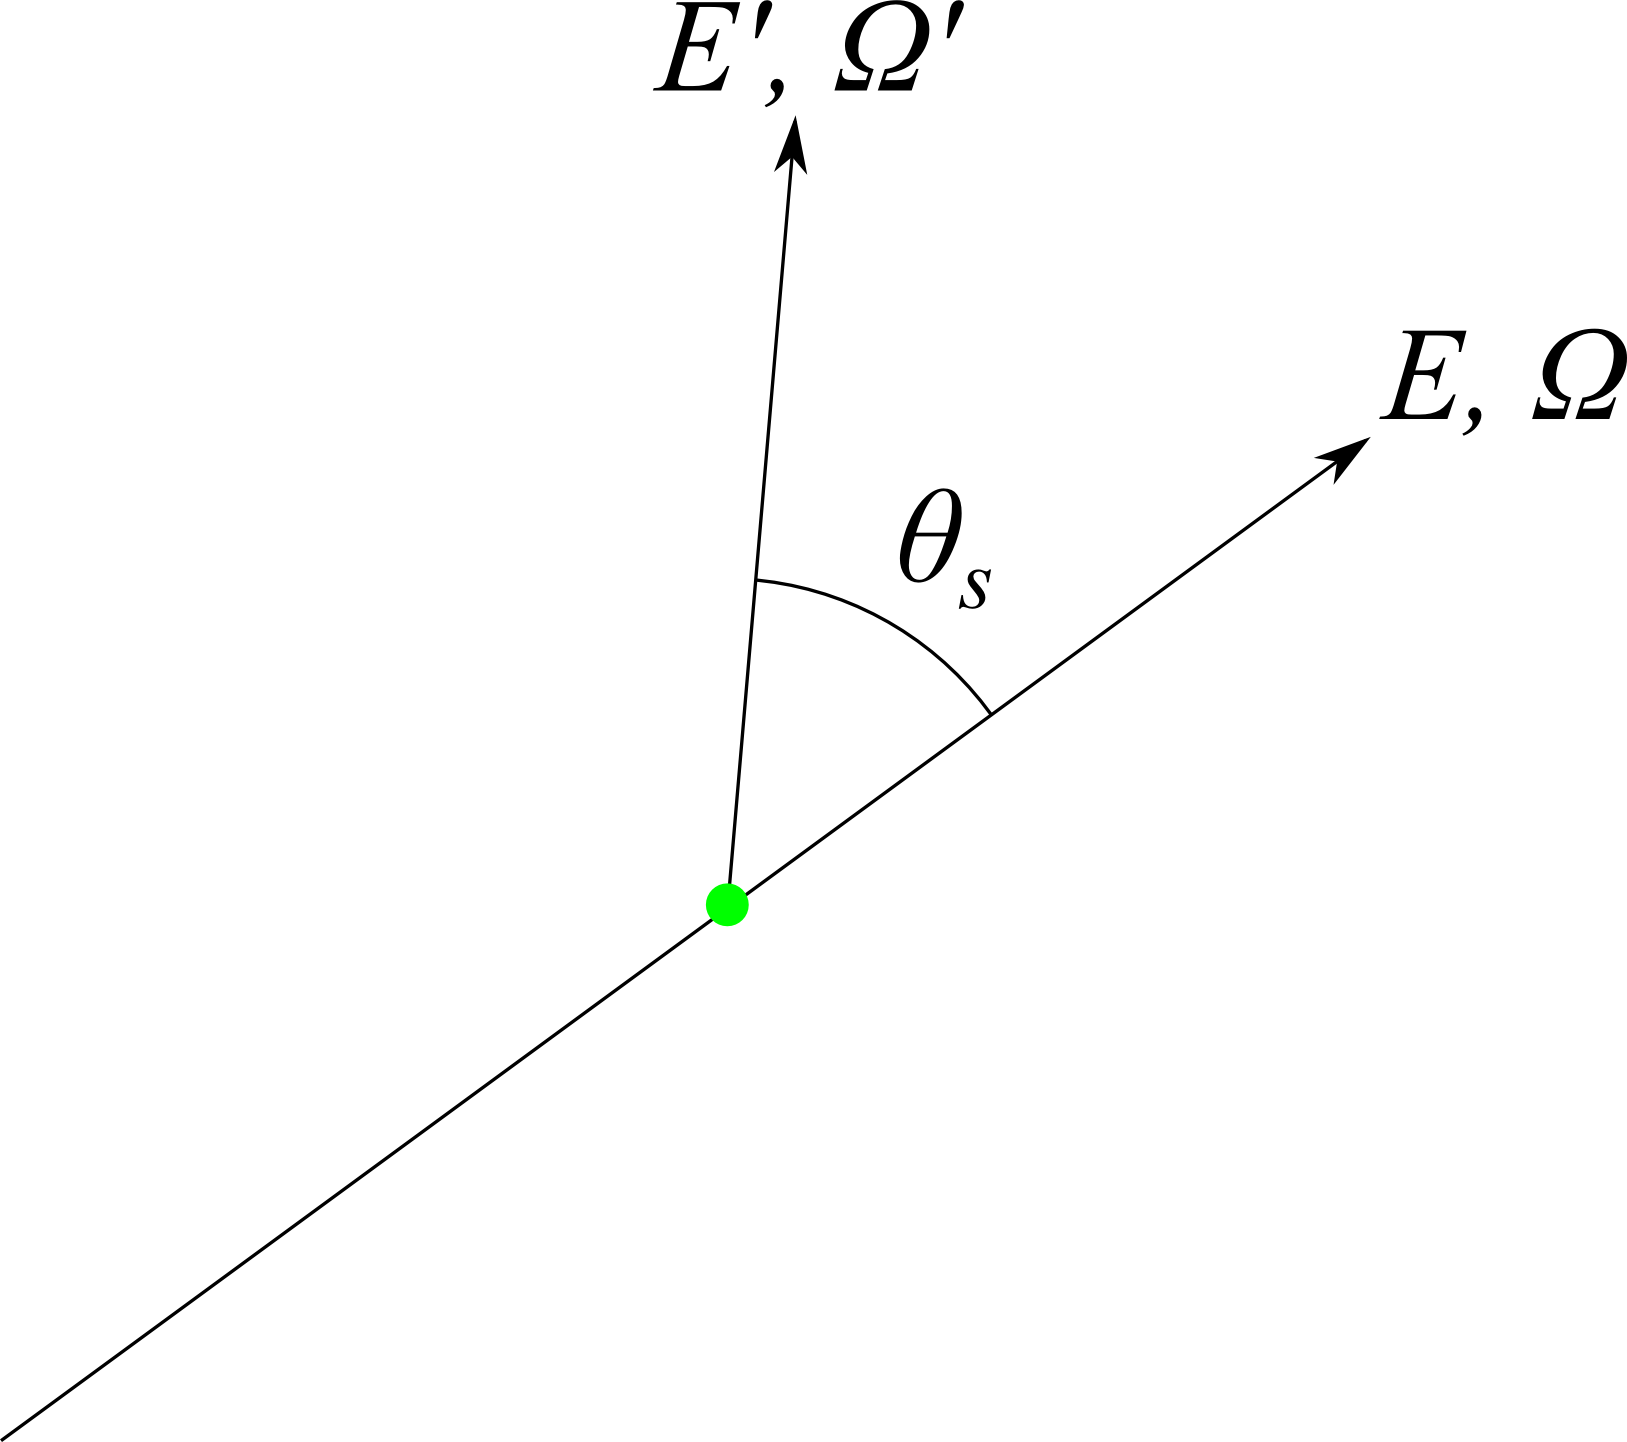
\includegraphics[width=3.75in]{figs/scat_ang}
  \end{center}
  \caption{The scatter angle. A photon at energy $E$ traveling in direction $\Omega$, hits a stationary atom, indicated by the green circle, and scatters into a new direction $\Omega'$ with a new energy $E'$.}
\label{fig:scat_ang}
\end{figure}%

The data files containing the scatter cross sections are distributed using a Legendre polynomial expansion. The use of a Legendre expansion removes the dependence on the quadrature from the data. This allows any quadrature to work with any dataset. A $l$-order Legendre polynomial is donoted by $P_l$. The anisotropic scatter cross section can then be rewritten as a Legendre expansion given in Eq.~\ref{eq:leg_1} where the scatter cosine is defined in Eq.~\ref{eq:scat_cos}

\begin{equation} \label{eq:leg_1}
\Sigma_{s, i, a, a'}^{g, g'} = \sum_{l=0}^L \frac{2l+1}{4 \pi}\Sigma_{s, i, l}^{g, g'} P_l(\mu_s)
\end{equation}

\begin{equation} \label{eq:scat_cos}
\mu_s = \Omega_a \cdot \Omega_{a'}
\end{equation}

\endinput
%%
%% End of file `chapmin.tex'.
